\documentclass[a4paper
,oneside,11pt]{article}
\usepackage[french]{babel}
\usepackage[utf8]{inputenc}
\usepackage[french]{babel}
\usepackage{fullpage}
\usepackage{xkeyval}
\usepackage{rotating}
\usepackage{amsmath}
\usepackage{amsfonts,amssymb}
\usepackage{float}
\usepackage{fancyhdr}
\usepackage{graphicx}
\usepackage{verbatim}
\usepackage{lastpage}
\usepackage{pstricks}
%\usepackage{aeguill}
\usepackage{color}
\usepackage{multicol}
\usepackage{mathenv}
\usepackage{amssymb}
\setlength{\headsep}{0.70cm}

%%%%%%%%%%%%%%%% Variables %%%%%%%%%%%%%%%%
\def\titre{Rapport\\Projet de Fin d'Année :\\Braille Music Compiler}
\def\titregauche{Projet de Fin d'Année}
\def\titredroite{Rapport de projet}
\def\filiere{informatique}
\def\annee{$2^{eme}$}  % $1^{ere}$, $2^{eme}$ ou $3^{eme}$
\def\anneescolaire{2011/2012}
\def\equipe{Pierrick Baudet \\ Pierre-Yves Canneill \\ David Dallago \\ Lun Jiang \\ Benjamin Lux \\Sara Rahhali\\Ali Slimani Houti}
\def\encadrant{Vinh-Thong Ta}
%%%%%%%%%%%%%%%%%%%%%%%%%%%%%%%%%%%%%%%%%%%


\pagestyle{fancy} \lhead{\textsc{\titregauche}} 
\rfoot{\textit{Ann\'ee \anneescolaire}}\rhead{\textsc{\titredroite}}\cfoot{\thepage/\pageref{LastPage}}
\renewcommand{\headrulewidth}{0.4pt}
\renewcommand{\footrulewidth}{0.4pt}

\newcommand{\HRule}{\rule{\linewidth}{0.5mm}}

\begin{document}

\begin{titlepage}

\begin{center}


% Upper part of the page
\begin{center}
\rotatebox{0}{\scalebox{1}[1]{
\includegraphics[width=5cm]{images/Logo_ENSEIRB-MATMECA.png}}}
\end{center}
~\\
~\\
~\\
\textsc{\LARGE ENSEIRB-MATMECA}\\[1cm]

\textsc{\Large {Fili\`ere \filiere, \annee ann\'ee}}\\[0.5cm]

% Title
\HRule \\[0.4cm]
{ \huge \bfseries \titre}\\[0.4cm]


\HRule \\[1.5cm]


% Author and supervisor
\begin{minipage}{0.4\textwidth}
\begin{flushleft} \large
\emph{Auteurs:}\\
\equipe
\end{flushleft}
\end{minipage}
\begin{minipage}{0.4\textwidth}
\begin{flushright} \large
\emph{Encadrant:} \\
\encadrant
\end{flushright}
\end{minipage}


\vfill

% Bottom of the page
{\large \today}

\end{center}

\end{titlepage}
\tableofcontents\thispagestyle{fancy}
\newpage
\section*{Introduction}\thispagestyle{fancy}
\addcontentsline{toc}{section}{Introduction}
\subsection*{Contexte}
Braille Music Compiler (BMC) est un outil de conversion du braille musical principalement destiné à l'usage de personnes aveugles ou malvoyantes. Il est capable d'interpréter une partition écrite en braille pour la convertir en une sortie audio qui peut par la suite être transformée en un fichier  MIDI ou MusicXML.\\

  BMC est actuellement à l'état de prototype, il est en cours de développement par Mario Lang, un autrichien non-voyant passionné par la musique et l'informatique.

  L'idée de développer un tel outil lui est venue lorsqu'il voulu jouer des partitions braille de musique classique. Souvent, il n'était pas sûr de bien interpréter certaine notes et s'est vite rendu compte que cette notation peut parfois porter à confusion. La notation Braille musicale est, en effet, assez complexe et peut parfois sembler ambiguë d'où l'utilité d'un programme qui servirait de référence en permettant d'écouter la note jouée. 
  
  Seulement la plupart des programmes disponibles sur le marché qui vont dans ce sens sont assez chers - coût moyen de 600 euros - et ne sont en général compatibles qu'avec Windows, ce qui limite fortement leur utilisation.\\
 
  M. Lang commença par travailler sur \textit{FreeDots}, un programme capable de convertir des partitions \textit{noires} de musique en partitions braille.\\
  Encouragé par le succès que rencontra ce premier programme, Il décida ensuite de se lancer dans la transcription inverse du braille musical, ce qui donna naissance au Braille Music Compiler. \\
  
  L'amélioration de l'utilisation du BMC notamment par implémentation d'une interface graphique nous a alors été proposée par Samuel Thibault, chercheur à l'INRIA et proche collaborateur du développeur du BMC. 
  
  
 
\subsection*{Problématique}
Le Braille Music Compiler est, pour l'instant, toujours en cours de développement. En effet, l'exécution de sa version actuelle requiert une certaine connaissance des outils informatiques, chose qui rend difficile son utilisation par un usager lambda.\\
L'intérêt de ce projet est donc d'améliorer cet outil de façon à ce qu'il devienne accessible à un plus large public. La mise en oeuvre d'une interface graphique permettrait en effet de rendre son utilisation plus intuitive.\\

  Étant principalement dédié à l'usage de personnes non(ou mal)-voyantes, l'interface graphique à implémenter doit donc répondre à un certain nombre de critères en termes d'accessibilité, elle doit être simple mais fonctionnelle.
  De plus, il serait intéressant que cette interface comporte aussi des fonctionnalités d'édition et de modifications de fichiers écrits en braille musical.
   
  Le BMC a aussi pour ambition de faciliter la collaboration entre voyants et non-voyants, en ce sens, l'interface devrait pouvoir à la fois afficher les partitions de musique écrites en braille et en \textit{noir} permettant ainsi à chacun des collaborateurs de pouvoir se repérer par rapport aux partitions de l'autre.    



\section{Organisation du travail}
%% Organisation du travail
\subsection{Méthode Scrum}
%% importances des tahces/ périodes de 3 semaines / selection des taches / encadrant pédagogique
Le responsable pédagogique de ce pfa, monsieur Ta, a préféré au classique cahier des charges une utilisation des méthodes agiles, plus précisément de la méthode \textit{scrum}.  Cette méthode semble être efficace
puisque aujourd'hui, nous avons bien avancé le projet et là où d'autre
groupes n'ont fait qu'un cahier des charges nous avons un début
d'application. Ce travail concret nous motive d'autant plus à nous
investire dans le projet. De plus, elle prépare le groupe à
l'entreprise puisque de nos jour, la plupart utilisent cette méthode.



\subsubsection*{Le Product Backlog}
La méthode \textit{scrum} place tous les collaborateurs du projet sur un pied d'égalité. Il faut tout d'abord créer un Product Backlog qui correspond à toutes les taches à effectuer pour la finalisation du projet.
Ce document doit être validé avec le client, puis ce dernier note les taches par ordre de priorité.

\subsubsection*{Un Sprint Backlog}
Ces dernières sont ensuites réparties en Sprint Backlog. Ce sont des périodes courtes durant lequelles l'équipe travaille sur certaines taches définies précédement. 
À la fin de chaque Sprint Backlog l'équipe présente sont travail sous forme concrète au client, sous forme d'un executable, de maquettes ou de toute autre forme.
Ceci est fait pour éviter au projet de partir dans une mauvaise direction et permet au client, dont les envies peuvent changer, de prendre part activement au projet.
La fin d'un sprint laisse place à une nouvelle réunion où sont définit les objectifs du sprint suivant.
Nous avons décidé de faire des Sprint d'une durée approximative de 3 semaines.

\subsubsection*{Les moyens de communication}
Afin de pouvoir travailer de façon efficace en groupe il est nécessaire de disposer d'outils spécialisés dans la gestion de projet.
Nous avons mis en place trois de ces outils.
Pour faciliter la communication au sein du groupe nous avons créé la liste \textit{pfa.bmc@listes.enseirb-matmeca.fr}. Cette liste est utilisable par tout le monde (membres du groupe, client, résponsable pédagogique) et envoye le mail aux seuls membres du groupe.
Pour gérer la méthode \textit{scrum} nous communiquons via \textit{Google docs} où nous avons créé une série de fichiers. Les principaux étant le Product Backlog, le détail des Sprint Backlog, le compte rendu des réunions avec l'encadrant et un ficher servant de tableau blanc.
Enfin nous avons mis en place un répertoire de travail sur \textit{Github} accécible en écriture aux membres du projet et visible par tous. Celui ci est accécible à l'adresse \textit{https://github.com/ddallago/pfa.bmc}.



\section{Spécification des besoins}

Le braille Music Compiler est d'abord conçu pour pouvoir convertir en sortie audio un fichier existant écrit en braille musical ainsi que pour permettre à son utilisateur d'apporter des modifications à un tel fichier ou d'en éditer un nouveau. Le BMC a, de plus, pour objectif de faciliter le travail commun de personnes voyantes et non-voyantes.

Le travail effectuer par l'équipe prends en compte ces deux aspects.

Les besoins du client nous ont été communiqués dans le document \textit{README.txt} sections \textit{User Interface(s)} et \textit{TODO}.

Après avoir rencontré M. Thibault, notre client local, et avoir discuté avec notre encadrant pédagogique M. Ta, nous avons pu déterminer les tâches que nous sommes en mesure de réaliser. 

Les sections qui suivent résument les actions que le délivrable devrait pouvoir accomplir.


\section{Besoins fonctionnels}
Le développeur du BMC souhaite que cet outil soit accessible au plus large public possible. Dans ce sens, le système d'exploitation sur lequel travaille l'utilisateur ne devrait pas être un obstacle à l'utilisation du Braille Music Compiler.\\

Nous décidons, dans un premier temps, de mettre en place une interface graphique sous Linux qui sera ensuite portée sous Windows.\\
 
Quelle que soit le système d'exploitation, la version finale de l'interface graphique devra pouvoir réaliser les actions suivantes, classées par ordre de priorité : \\

\begin{itemize}
  \item \textbf{Ouvrir un fichier :} affichage sur le programme principal du contenu d'un fichier écrit en braille musical sélectionné via une fenêtre de sélection.\\
  \item \textbf{Enregistrer un fichier :} enregistrement sur le disque dur du fichier ouvert en écrasant sa copie existante (se trouvant au même emplacement).\\
  \item \textbf{Fermer l'application :} fermeture du fichier ouvert en demandant la confirmation de sauvegarde des modifications éventuelles.\\
  \item \textbf{Éditer un fichier braille :} ce point regroupe toutes les fonctionnalités habituellement proposées par un éditeur de texte comme les actions de copier, coller, couper un partie du texte ainsi que les actions de sélection de lignes et paragraphes.\\
  \item \textbf{Écouter une sélection :} lecture des notes sélectionnées.\\
  \item \textbf{Colorer le texte braille :} coloration du texte afin de faciliter à la personne voyante (collaborant avec un non-voyant) de se repérer par rapport aux notes écrites en braille musical.\\
  \item \textbf{Afficher la note en cours :} déplacement du curseur au fur et à mesure que les notes sont jouées pour que l'utilisateur puisse savoir à quel son correspond quelle note.\\
% \item \textbf{Afficher partition visuelle :}\\
  \item \textbf{Numéroter les mesures :} autre fonctionnalité pour faciliter la collaboration entre voyant et non-voyant, la numérotation des mesures permet à chacun de se repérer par rapport aux notes de l'autre.\\
\end{itemize}

\section{Besoins non-fonctionnels}
En plus des besoins fonctionnels auxquels doit répondre le projet, ce dernier doit satisfaire les point suivants:\\
\begin{itemize}
\item \textbf{Portabilité :} le code doit être écrit de façon à pouvoir en réutiliser la plus grande portion lors du portage sur d'autres systèmes d'exploitation.\\
\item \textbf{L'extensibilité :} le délivrable doit répondre à ce critère car il est susceptible d'être modifié par M. Lang.\\
\item \textbf{Autonomie :} l'utilisation du travail rendu ne devrait pas demander de mise en place lourde, et son installation doit être facile.\\
\item \textbf{Modularité :} le code doit être réparti en modules, afin de garantir la possibilité de réutiliser le code par le client ainsi qu'une meilleure gestion des erreurs. De plus, l'injection de nouvelles classes ou méthodes dans le projet doit être le plus possible indépendante du code du client.\\
\item \textbf{Documentation :} le code doit être documenté en anglais pour faciliter sa compréhension ainsi que sa réutilisation par le client.\\

\end{itemize}



\section{Travail effectué}
%% Travail effectué
\section{BMC}

BMC, "Braille music compiler" est un programme qui se veut de transformer un fichier écrit en "Braille Music" en un autre langage utilisable par d'autres applications. La difficulté est que le langage "Braille Music" possède beaucoup d'ambiguïtés, en effet par exemple pour connaître la note exacte en cours, il est nécessaire de savoir quelles ont été les notes précédentes. A l'heure actuelle le programme arrive correctement à compiler le langage "Braille Music" en un langage Abstrait qui lui ne possède aucune ambiguïté. Ce langage abstrait peut être converti en n'importe quels formats de musique. Par exemple : 
\begin{itemize}
\item MIDI
\item MusicXML
\item lilypond
\end{itemize}
\begin{figure}[!h]
  \centering
  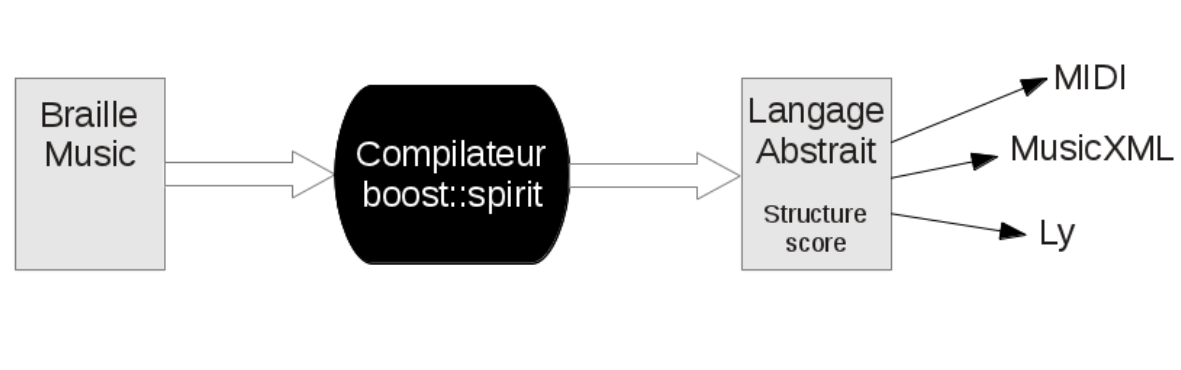
\includegraphics[scale=0.4]{images/fonction-bmc.png}
  \caption{Schéma visuel du fonctionement de BMC}
  
\end{figure}

Notre travail est donc d'implémenter ses modules de convesion. Pour cela il est nécessaire de comprendre comment est conçu le langage Abstrait. Après la compilation du "Braille Music", l'ensemble des données sont stockées dans une structure nommée "score". Cette structure est une multitude de vecteurs imbriqués les uns dans les autres. Voici le code de la strucure suivi d'une représentation visuel :

\begin{verbatim}
typedef boost::variant<note, rest, chord, value_distinction, hand_sign, simile, barline>;
typedef std::vector<sign> partial_voice;
typedef std::vector<partial_voice> partial_measure;
typedef std::vector<partial_measure> voice;
struct measure : locatable
{
  boost::optional<unsigned> ending;
  std::vector<voice> voices;
};
typedef std::vector< boost::variant<measure> > staff;
typedef std::vector<staff> part;
struct score {
  boost::optional<time_signature> time_sig;
  std::vector<part> parts;
};
\end{verbatim}

\begin{figure}[!h]
  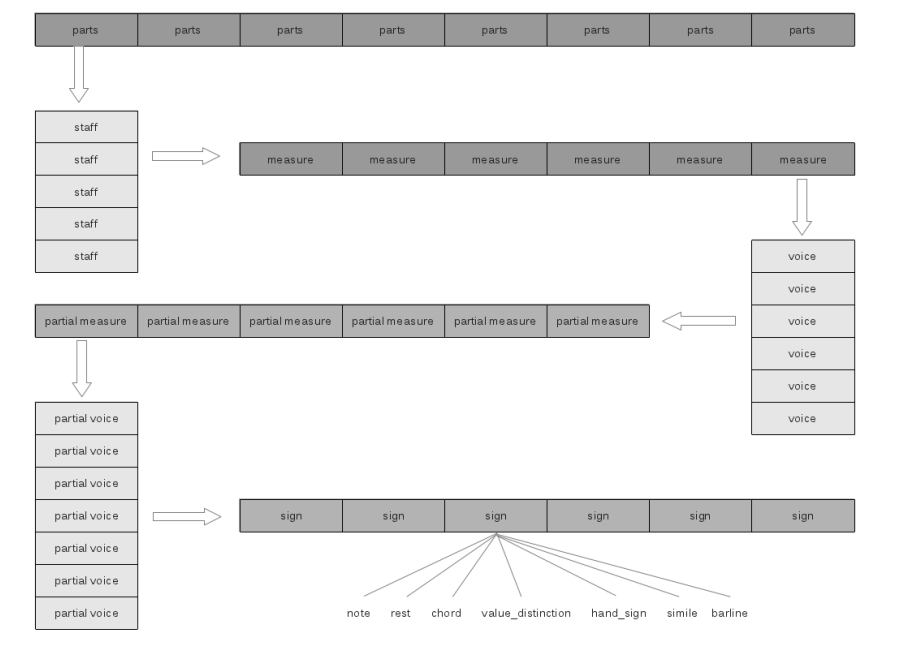
\includegraphics[scale=0.8]{images/bmc-score.png}
  \caption{Représentation de la structure score}
\end{figure}

Il est donc maintenant plus facile d'expliquer la structure \textit{score}. Un fichier de musique braille peut donc se diviser en plusieurs parties (parts). Chaque partie possède un ou plusieurs "staff". Un "staff" n'est autre que la portée, typiquement si le compositeur écris une partition de musique pour piano il y aura deux portées. Chaque portée possède un nombre de mesures. Si la musique composée est polyphonique il y aura plusieurs voix ("voices"). Une voix est ensuite divisée en mesures partielles ... ( // TODO )).


\begin{figure}[!h]
  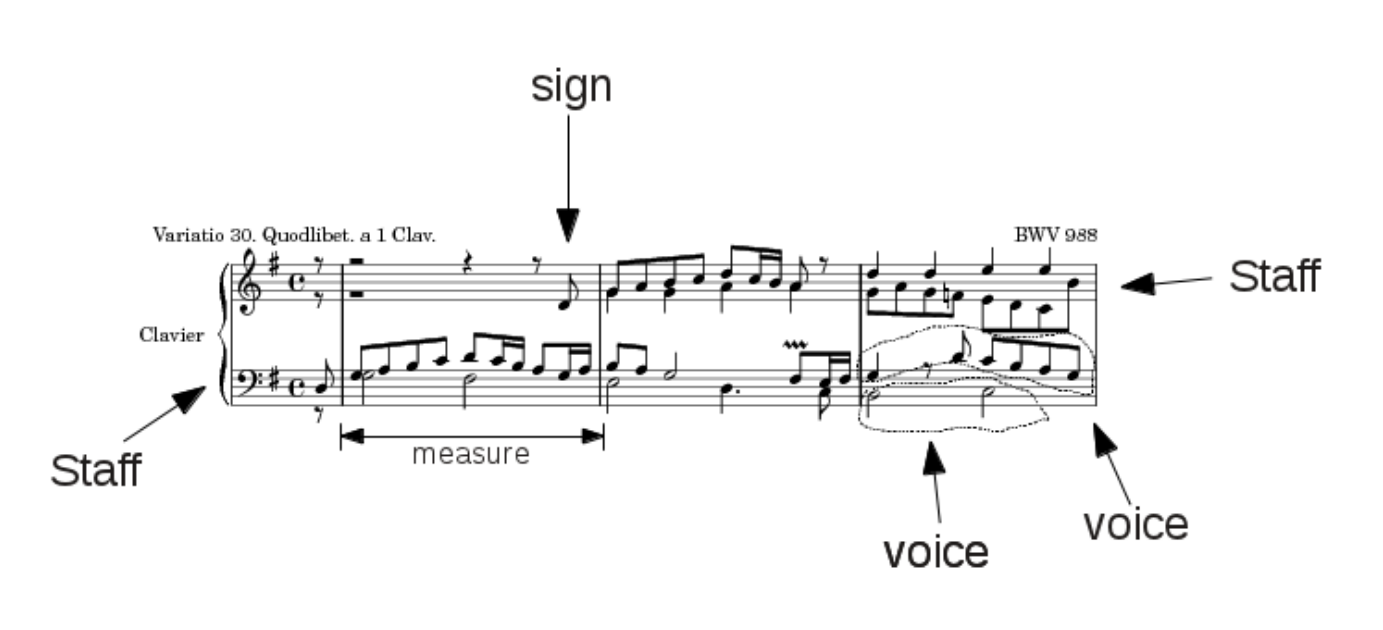
\includegraphics[scale=0.4]{images/score-visu.png}
  \caption{Un petit exemple visuel}
\end{figure}

Avant de se mettre à faire la conversion du langage abstrait vers un format de musique conventionel nous avons d'abord créé les classes de base que nous devrons utiliser pour effectuer les différentes conversions. On procède à un affichage sur le terminal dans un premier temps.

\begin{verbatim}
./bmc < input/bwv988-v30.bmc 

 r1/8  r1/8 >  |   r1/2  r1/4  r1/8 D 5 >   r1/1 >  |  G 5 A 5 B 5 C 6 D 
6 C 6 B 5 A 5  r1/8 >  G 5 G 5 A 5 A 5 >  |  D 6 D 6 E 6 E 6 >  G 5 A 5 G 
5 F 5 Natural  E 5 D 5 C 5 B 5 >  |  B 5 A 5 G 5 G 5 G 5 D 5 >  |   r1/2 
 r1/4  r1/8 D 6 >  G 5 A 5 B 5 C 6 D 6 C 6 B 5 A 5 D 6 >  G 5 G 5 A 5 A 5 > 
\end{verbatim}

\section{Interface graphique}

L'un des critères essentiels de ce projet est l'accessibilité. Par
conséquent, nous avons choisi d'utiliser la bibliothèque GTK+ pour
l'interface graphique sur plateforme linux. En effet, cette
bibliothèque est compatible avec les lecteurs d'écran des systèmes
linux.


\subsection*{Forme}
L'interface graphique est très classique: elle présente une barre de
menu, une barre de raccourcis ainsi que les raccourcis naturels,
encore en cours d'implémentation. La fenêtre se divise en deux
parties: la premiere partie sert pour l'utilisateur malvoyant à éditer les partitions brailles. La
deuxième partie sert à l'utilisateur voyant à avoir une partition
classique.

\begin{center}
\begin{figure}[!h]
  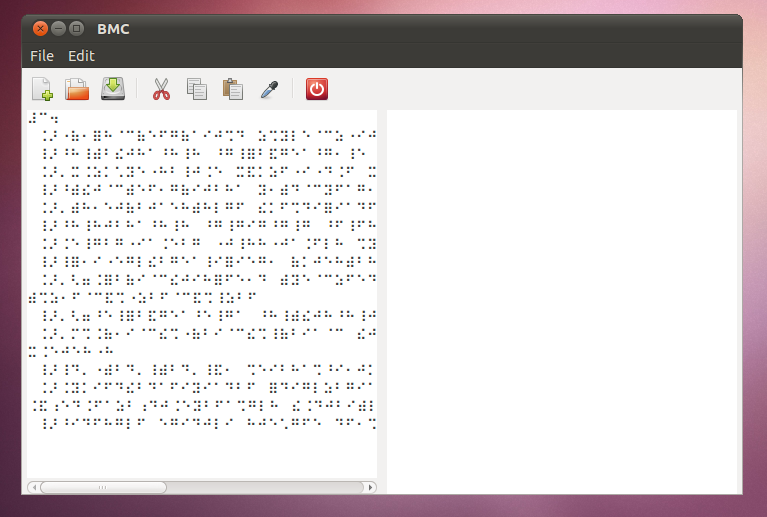
\includegraphics[scale=0.65]{images/linux_gui.png}
  \caption{Représentation de la structure score}
\end{figure}
\end{center}



\subsection*{Fonctionnalités}
Le prototype réalisé comporte tous les fonctionnalités de base d'un
éditeur de texte. Il permet de créer un nouveau fichier, d'ouvrir un
fichier, d'enregistrer un fichier et d'enregistrer le fichier courant
sous un autre nom. Il permet aussi d'éditer les textes avec les outils
classiques comme copier, couper, coller, séléctionner du texte.
\\ Non seulement, toutes ces fonctions sont accessible depuis la barre
de menu et/ou la barre d'outils, elles sont également toutes associées
à des raccourci clavier. Les raccourcis utilisés sont très
classiques. Par exemple, Ctrl+O pour ouvrir, Ctrl+C pour copier et
Ctrl+V pour coller.
\\ Le prototype possède aussi une procedure de
sécurité qui consiste à vérifier si le fichier en cours d'édition est
sauvegardé ou non et propose à l'utilisateur d'enregistrer son
fichier lorsque l'utilisateur tente de créer un nouveau fichier,
d'ouvrir un autre fichier ou encore de quitter le programme.


\subsection{Programmation évenementielle}

La programmation événementielle est la base de tout programme interactif.
Il fonctionne sur le principe \textit{action \rightarrow réaction}. L'exemple 
immédiat est le clic sur un bouton (\textit{action}) qui déclenche (\textit{réaction}) 
l'appel à une fonction, dite \textit{CALLBACK}.

GTK+ gère lui-même ces différentes actions (signaux) pour tous les widgets.
Ceux-ci captent l'action de l'utilisateur (\textit{e.g} le clic}), émettent 
un signal, GTK+ reçoit le signal et sait alors quelle fonction \textit{CALLBACK} 
appeller.

La tâche du développeur est grandement simplifiée par l'utilisation des 
bibliothèques GTK+ : la fonction à utiliser a pour prototype
\begin{verbatim}
gulong g_signal_connect(gpointer *object, const gchar *name, GCallback func, gpointer func_data);
\end{verbatim}
où 
\begin{itemize}
\item $object$ est un pointeur vers le widget contenant le bouton (\textit{e.g} $G\_OBJECT(editor->window)$) ;
\item $name$ est le nom de l'évènement (\textit{e.g} $"destroy"$) ;
\item $func$ est la fonction \textit{CALLBACK} (\textit{e.g} $G\_CALLBACK(gtk\_main\_quit)$) ;
\item $func\_data$ est un paramètre donné à $func$.
\end{itemize}

\\

Une autre méthode permet d'associer le clic d'un bouton à une action.
Dans le cadre d'une boîte de dialogue proposant plusieurs choix (\textit{e.g} : Voulez-vous 
sauvegarder avant de quitter ?), la création de ce $dialog$ permet au développeur de décrire son 
fonctionnement. Suite à la création d'un nouveau widget $dialog$, contenant les boutons OUI et NON 
$GTK\_BUTTONS\_YES\_NO$, il suffit de lancer ce widget et stocker sa valeur de retour dans une variable :
\begin{verbatim}
	gint resp=gtk_dialog_run (GTK_DIALOG (dialog));
\end{verbatim}
Il ne reste plus qu'à dissocier :
\begin{verbatim}
	if ( resp == GTK_RESPONSE_YES)
		_save();
	else if( resp == GTK_RESPONSE_NO)
		_quit();
\end{verbatim}




\section{Bibliotèque BOOST}

Lors de notre analyse du langage abstrait et ce en scrutant de plus près le code source du \textit{Braille Music Compiler} nous étions amenés à étudier la bibliothèque BOOST  qui est un ensemble de bibliothèques C++ gratuites et portables. BOOST est très riche et fournit un large choix de bibliothèques, mais nous ne préciserons que celles utilisées pour le stockage de la musique sous forme de langage abstrait.


\subsection*{Boost.Variant}

Le Boost.Variant est une sorte de type \textit{somme}. Il s'agit en fait de décomposer un type donné en plusieurs sous-types. Une instance de ce type donné peut être obtenue par une valeur de ses sous-types, mais pas deux types à la fois. Ce qui peut être assimilé à une \textit{union}. Cependant, en \textit{C} et \textit{C++} le type \textit{union} ne permet pas de gérer des classes dès qu'elles ont un constructeur ce qui est rendu possible grâce au Boost.Variant en \textit{C++}.

Donc contrairement à un \textit{std::vector} en C++ qui offre des éléments \textit{multi-valeur, type unique}, le \textit{boost::variant} offre des éléments \textit{multi-type, valeur unique}.

%Dans le cadre de notre projet, le boost variant nous permet de

\subsection*{Boost.rational}

Le langage C++ offre plusieurs possibilités pour stocker des nombres, des entiers naturels aux réels et ce en les approximant par différents types : unsigned int, int, float... La bibliothèque boost.rational permet de représenter un nouveau groupe de nombres : les nombres rationnels.

Au niveau implémentation le type Boost.rational est constitué de deux nombres de type entier, qui représente le numérateur et le dénominateur. De cette façon, cela permet d'avoir une meilleure précision de calcul et de faciliter l'implémentation.






\section*{Conclusion}\thispagestyle{fancy}
\addcontentsline{toc}{section}{Conclusion}

\chapter{Conclusion}

Ce premier rapport ainsi que le \textbf{Product Backlog} en annexe résultent des différents rendez-vous avec le client local ainsi que les multiples réunions que l'équipe a eu avec l'encadrant pédagogique.\\
Ces deux documents font état de l'avancement du projet à ce jour.\\

La réalisation du projet étant amenée à avancer, certains points de ce document sont susceptibles d'être modifiés. Cependant, les points fondamentaux de la conception du projet se doivent d'être respectés.\\




%\section{Glossaire}
%%%


\end{document}

